\chapter{Team 5 Agent Design}\label{team_5_agent_design}

The Team 5 agent operates on the basis that upon entering the tower, the need to ensure its own survival is its only aim and therefore the agent should maximise its own HP whenever given the opportunity to do so. When there is not enough food to fully satisfy all agents, the agent alters its behaviour to best increase its long-term survival.

This situation can be thought of as a `hawk-dove' game where it is beneficial for all agents to take less food but any single agent who does so is worse off if no other agents follow suit. Communication is key to breaking out of this situation. This agent will attempt to establish relationships with surrounding agents -- the agent has parameters to judge other agents and also attempts to learn about the tower -- and encourage behaviours that benefit the overall tower utility.

However, the agent will also be influenced by the behaviour of agents around it: if other agents are selfish then it will also be selfish. This can be thought of as a `tit-for-tat' strategy, but with enough HP, agents will be willing to `make the first move', with the insurance that if others do not follow then they have some buffer time to re-establish their own selfish behaviour.

An agent will maintain a low HP only if it is confident that other agents will allow it to survive by leaving enough food, through the signing of treaties to build trust. A tower that consists solely of Team 5 agents would require those at the top to be willing to decrease their own short-term satisfaction in order to give the best chance of survival for all agents, and trust others to do the same upon reshuffling.

Section \ref{sec:team5-overview} provides an overview of the agent's parameters and strategy, Section \ref{sec:team5-messaging} describes the agent's communication strategy, Section \ref{sec:team5-memory} describes how the agent stores its social network and how it judges other agents, and Section \ref{sec:team5-treaties} describes how the Team 5 agent utilises treaties. Finally, Section \ref{sec:team5-experimentation} contains analysis of this agent including how it performs in a tower consisting of itself alone as well as together with other agent types and Section \ref{sec:team5-conclusion} provides summarising remarks regarding the implementation of this agent type.

\section{Agent Overview}
\label{sec:team5-overview}

\ToDo{Give better description of Run function}

The strategy employed by this agent aims to maximise its chances of survival while also considering those who have helped the agent in the past.

At the beginning of each day, the agent's `personality' is updated using various parameters stored from previous days. These personality parameters are shown in Table \ref{tab:team5-personality}. Each of these parameters are linked and contribute to the calculation of how much food an agent will attempt to eat.

\begin{table}
    \centering
\begin{tabular}%
    {| >{\raggedleft\arraybackslash}p{0.25\linewidth} | %
    >{\raggedright\arraybackslash}p{0.65\linewidth} | %
    }
    \hline
    Selfishness          & Ranges from 0 to 10. Determines how much the agent will act for their own survival as opposed to the best interests of the surrounding agents\\
    \hline
    Last Meal            & How much the agent ate in their last meal\\
    \hline
    Days Since Last Meal & How many days since the agent last ate\\
    \hline
    % HP After Eating      & \\
    % \hline
    Aim HP               & Defines the goal HP the agent would like to reach at the end of the day\\
    \hline
    Attempt Food         & The amount of food the agent will attempt to take from the platform\\
    \hline
    Messaging Counter    & Determines which message type to send to which floor \\
    \hline
    % Treaty Send Counter  & \\
    % \hline
    % Attempt To Eat       & \\
    % \hline
    Leadership           & A threshold value required for the agent to propose treaties\\
    \hline
    Social Memory        & Stores the information the agent learns about other agents, as well as its opinion of them (see Table \ref{tab:team5-memory})\\
    \hline
    Surrounding Agents   & A list of the agent's neighbours\\
    \hline
\end{tabular}
\caption{The personality parameters of Team 5's agent}
\label{tab:team5-personality}
\end{table}

At the start of each tick, the agent checks to see if it has received any messages and if so, will respond to these\footnote{Note that an agent can receive and respond to only one message per tick.}. The agent then sends out messages to other agents. The mechanism for messaging is described in Section \ref{sec:team5-messaging}.

\section{Messaging}\label{sec:team5-messaging}
Collaboration between different agents operating in a system requires communication. The motivation for messaging is to improve the agent's understanding of its surroundings, enable the building of mutually beneficial relationships, and introduce collaboration and agreement between parties.

\subsection*{Strategy}\label{sec:team5-messaging-strategy}
The agent's approach to messaging is to adopt a ``passive observer'' role focussed on gathering information about other agents to organise itself with these agents in the tower. With more information at its disposal, the agent can make more informed decisions to balance its own individual utility with the collective utility of the agents in the tower.

The agent sends three types of messages to each of the agents residing one or two floors above and below its own floor; it therefore takes 12 ticks to send all of its messages. These messages ask for the HP, intended food intake, and actual food intake of other agents. The decision of which message type to send to which floor is controlled by the \texttt{Messaging Counter} described in Table \ref{tab:team5-personality}. This counter is incremented each tick, and reset either every 25 ticks or at the end of each day, whichever comes first. This ensures that the agent is requesting up-to-date information regularly for use in its decision making.

The order of sent messages is:
\begin{enumerate}
    \item Ask for an agent's HP
    \item Ask for an agent's previous food intake
    \item Ask for an agent's intended food intake
\end{enumerate}
The Team 5 agent first targets the agent immediately below it, then the agent immediately above, then two floors below, and finally the agent two floors above.

In addition to sending out requests for information, the agent also accepts any state messages it receives even if it did not ask for them, so that it can gain the largest amount of knowledge that it can. This includes messages where the agent is not the intended recipient: in this case the Team 5 agent will read the information contained in the message before passing it on.

\section{Social Memory}\label{sec:team5-memory}
The agent stores the information gained from communication in its `memory': the information stored by this data structure is shown in Table \ref{tab:team5-memory}.

\begin{table}
    \centering
    \begin{tabular}%
        {| >{\raggedleft\arraybackslash}p{0.25\linewidth} | %
        >{\raggedright\arraybackslash}p{0.65\linewidth} | %
        }
        \hline
        Agent ID & An agent's unique ID\\
        \hline
        Agent HP & The agent's last known HP level\\
        \hline
        Food Taken & The amount of food the agent last took\\
        % \hline
        % Intended Food Intake & The amount of food the agent intends to take\\
        \hline
        Favour & The Team 5 agent's opinion of this agent\\
        \hline
        Days Since Last Seen & The number of days since the last message from this agent\\
        \hline
    \end{tabular}
    \caption{Team 5 Agent Memory}
    \label{tab:team5-memory}
\end{table}

This memory allows the agent to construct a social network of agents in the tower and evaluate others based on these parameters. This consequently leads to the idea of favour, a metric the Team 5 agent uses to judge other agents. If more than five days have passed since the agent's last interaction with another agent, then the knowledge gained of that agent is reset, with the favour value being kept. This prevents the agent from using out-of-date information in its calculation while still allowing the opinion formed of the agent to be retained indefinitely.

\subsection*{Favour}\label{sec:team5-favour}
The favour metric quantifies the agent's opinion of others in the tower. It is bounded between 0 and 10, and in a single tick can either increase by 1, decrease by 3, or stay the same:

\begin{align*}
    \texttt{hpScoreOther} &= -1 \times \frac{\texttt{otherHP}^{1.7} \times \texttt{foodTaken}^{1.3}}{\texttt{maxHP}^3}\\
    \texttt{hpScoreSelf} &= \frac{\texttt{ownHP}^{1.7}\times\texttt{ownAttemptFood}^{1.3}}{\texttt{maxHP}^3}\\
    \texttt{judgement} &= 100 \times (\texttt{hpScoreOther} + \texttt{hpScoreSelf})\\
    \texttt{unboundedFavour} &= \begin{cases}
        \texttt{originalFavour} + 1, \quad\hfill \texttt{judgement} &> 0.075\\
        \texttt{originalFavour} + \max{\left(\frac{\texttt{judgement}}{2}, -3\right)}, \quad\hfill\texttt{judgement} &< -2
    \end{cases}\\
    \texttt{favour} &= \begin{cases}
        0, \quad\hfill \texttt{unboundedFavour} &< 0\\
        \texttt{unboundedFavour}, \quad 0 \leq \texttt{unboundedFavour} &\leq 10\\
        10, \quad\hfill \texttt{unboundedFavour} &> 10
    \end{cases}\\
\end{align*}

We have designed the favour calculation in such a way that means positive changes in favour occur slowly while negative changes in favour can occur quickly; this was done to design an agent which builds trust slowly over time but will lose trust quickly when other agents behave in a way deemed to be detrimental to the collective good. The exponents of 1.7 and 1.3 were obtained using trial and error to see which values gave the most desired performance.

Measuring favour allows the agent to act according to how other agents are behaving around it, while taking on a passive conformist approach to decision making. If the agent views others around it more favourably, then it eats less food and aims for a lower HP in hopes of improving collective utility. The agent is also more likely to propose treaties to, and accept treaties from, highly favoured agents.

For agents which have low favour, the Team 5 agent maintains its passiveness and does not ``punish'' them by, for example, taking more food than is necessary. The effect of ``punishing'' an agent propagates to all floors below the agent and is therefore deemed an inappropriate course of action. Instead, the agent strives to behave positively if surrounding agents also demonstrate positive behaviour.

It should also be noted that while the Team 5 agent computes favour for agents both above and below its floor, a positive favour value for agents above is helpful to that agent only if they are moved to a floor below the Team 5 agent following a reshuffle: this is because there is no way to reward the behaviour of an agent above you in the tower.

\section{Treaties}\label{sec:team5-treaties}
The Team 5 agent's treaty strategy consists of three main parts:
\begin{enumerate}
    \item Deciding whether to accept or reject proposed treaties
    \item When to propose a treaty
    \item What to propose as a treaty
\end{enumerate}

\subsection*{Responding to Proposed Treaties}\label{sec:team5-treaties-response}
A proposed treaty is always rejected if:
\begin{itemize}
    \item It conflicts with any other active treaties. A treaty is considered to conflict with another treaty if they could ever cause the agent to take incompatible actions. For example, an agent cannot leave more than five units of food and fewer than four units of food at the same time.
    \item It is badly formed. For example, a treaty which requires the agent to leave more than 100\% of the food on the platform is badly formed.
    \item It requires agents to leave less than a certain amount of food on the platform, as this is never advantageous to the tower as a whole.
    \item It requires the agent to leave an exact amount of food on the platform, as this would result in all but one of the agents signed up to the treaty to take no food each day.
    \item It makes a request based on low HP, low amounts of food on the platform, or a low floor, as in these conditions the agent will already be desperate for survival, so will not want to be further constrained by a treaty.
    \item It makes a request based on HP where the threshold is within the ``weak'' or ``critical'' HP bands, as this means the agent could become critical or die as a result of following the treaty.
    \item It would require the agent to take less food than is required to avoid entering the ``critical'' HP band.
\end{itemize}
If the treaty does not meet any of the above conditions, the \texttt{decision} value is then computed as:
\[\texttt{decision} = 6 - \texttt{selfishness} + \texttt{proposerFavour} - \frac{\texttt{treatyDuration}}{3}\]

This calculation is based on the following considerations:
\begin{itemize}
    \item Selfish agents will always be less likely to sign treaties
    \item The proposing agent is more likely to be trusted if the receiving agent views them more favourably
    \item Longer treaties are viewed more negatively because factors such as the receiving agent's opinion of the proposer and the agent's selfishness can change over time, meaning the same treaty could be viewed less favourably in future. Therefore, the agent should avoid constraining its actions to satisfy an agent of which it could form a negative opinion.
\end{itemize}

If the \texttt{decision} value is positive, the treaty is accepted.

\subsection*{Proposing Treaties}\label{sec:team5-treaties-proposal}
At the start of each day, the agent checks whether it has become a `leader': if it has, then the agent proposes a treaty. Whether an agent becomes a leader or not is based on:
\begin{itemize}
    \item The agent's selfishness: a selfish agent is less likely to propose treaties
    \item The agent's floor: agents higher up in the tower are more likely to propose treaties. This is because an agent's floor is the only indicator of social hierarchy in the tower, as those at the top can choose the amount of food they eat and therefore control the amount of food available to those below them. This control means these agents are in a better position to effect change.
    \item The agent's \texttt{leadership} threshold: this is randomly set during the agent's initialisation and those with a lower leadership threshold are more likely to become leaders.
\end{itemize}
The leadership value is calculated by:
\[ \texttt{leadership} = x - \texttt{selfishness} - \texttt{agentFloor}\]
The variable $x$ is a random number between 3 and 12, inclusive. If \texttt{leadership} is greater than the agent's leadership threshold, then the agent becomes a leader and proposes a treaty.

The proposed treaty is always that agents whose HP is greater than or equal to a certain value should always leave 100\% of the food on the platform, and always lasts for five days. The threshold value for HP is calculated using Equation \ref{eq:team5-treaty-hp-threshold}. Note that in this equation, \texttt{WeakLevel} refers to the threshold between the ``critical'' and ``weak'' HP states.

\begin{equation}\label{eq:team5-treaty-hp-threshold}
    \texttt{hpThreshold} = \texttt{aimHP} - \frac{\texttt{aimHP} - \texttt{WeakLevel}}{10}\times\left(\texttt{leadership} - \texttt{leadershipThreshold}\right)
\end{equation}

It was decided that of the available treaty types, treaties that limit HP were the most suitable for composing resource management-based agreements between agents. This is because treaties based directly on quantities of food make it difficult to construct treaties that control each agent's food intake in a fair manner. While food is the main reseource in the tower, we can view HP as a secondary resource given that it is directly affected by food and reflects the allocation of this main resource.

\section{Experimentation}\label{sec:team5-experimentation}
This section focuses on the agent's performance and how this varies with changes in its environment.

\subsection*{Homogeneous Tower Experiments}
To evaluate the self-organisation abilities of the Team 5 agent, simulations were run with the agent in variations of a homogeneous tower, i.e., a tower that contains agents of only one type. The agent has been evaluated on three main metrics:
\begin{enumerate}
    \item The number of deaths
    \item The average utility
    \item Whether self-organisation was achieved.
\end{enumerate}
Self-organisation has been defined in this case to be when all agents take only what they need to survive and there are little to no deaths beyond a certain point in time.

\subsubsection*{Food Per Agent On Platform}
The baseline experiment for testing was to vary the amount of food per agent available on the platform; it was expected that having more food available would result in fewer deaths. In this experiment, simulations were run for 100 simulation days, with a reshuffle period of 7 days and 50 agents in the tower and repeated three times, with the average of these runs taken. Figure \ref{fig:team5-deaths-utility-food-per-agent} shows that the number of deaths decreases and average utility increases as we increase the amount of food available.

When the ratio of food to agent is greater than 9, the agents are able to self-organise within 100 days, and typically do so within 70 days. When food availability was less than this, the agents did not achieve self-organisation. However it was interesting to observe that more treaties were accepted than rejected. This shows that the agents recognise the need to self-organise and are willing to make attempts to do so. It is possible that they did not achieve self-organisation in this case because agents died too quickly to reach agreements among enough agents for this to be successful.

\begin{figure} % Number of Deaths and Average Utility vs Available Food Per Agent
    \centering
    \begin{minipage}{0.6\textwidth}
        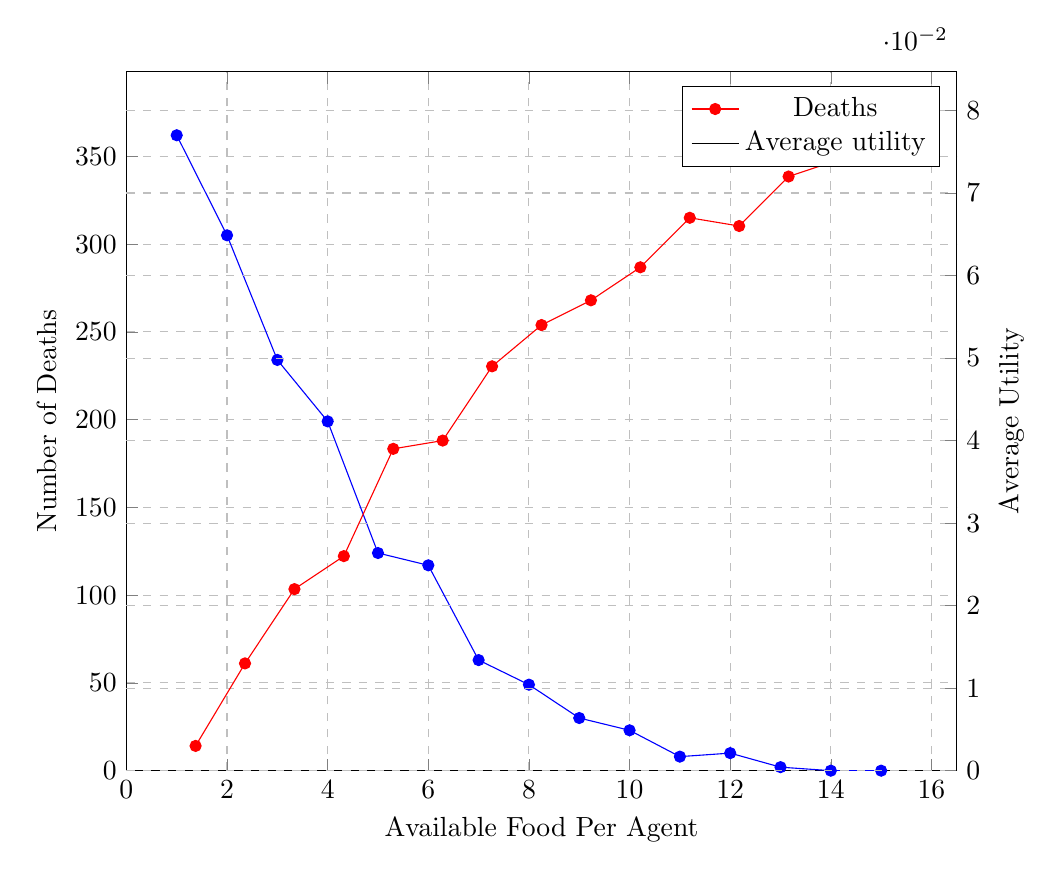
\begin{tikzpicture}
            \begin{axis}[
                width=\textwidth,
                axis y line*=left,
                ymin=0,
                xmin=0,
                xlabel=Available Food Per Agent,
                ylabel=Number of Deaths,
                ymajorgrids=true,
                xmajorgrids=true,
                grid style=dashed,
            ]
            \addplot[mark=*,blue]
                coordinates{
                    (15, 0)
                    (14, 0)
                    (13, 2)
                    (12, 10)
                    (11, 8)
                    (10, 23)
                    (9, 30)
                    (8, 49)
                    (7, 63)
                    (6, 117)
                    (5, 124)
                    (4, 199)
                    (3, 234)
                    (2, 305)
                    (1, 362)
                }; \label{leg:team5-food-per-agent-deaths}
            \end{axis}
            
            \begin{axis}[
                width=\textwidth,
              axis y line*=right,
              axis x line=none,
              ymin=0,
              ylabel=Average Utility,
              ymajorgrids=true,
              xmajorgrids=true,
              grid style=dashed,
            ]
            \addplot[mark=*,red]
                coordinates{
                    (15, 0.077)
                    (14, 0.074)
                    (13, 0.072)
                    (12, 0.066)
                    (11, 0.067)
                    (10, 0.061)
                    (9, 0.057)
                    (8, 0.054)
                    (7, 0.049)
                    (6, 0.04)
                    (5, 0.039)
                    (4, 0.026)
                    (3, 0.022)
                    (2, 0.013)
                    (1, 0.003)
                }; \label{leg:team5-food-per-agent-utility}
                \addlegendimage{/pgfplots/refstyle=leg:team5-food-per-agent-deaths}\addlegendentry{Deaths}
                \addlegendimage{/pgfplots/refstyle=leg:team5-food-per-agent-utility}\addlegendentry{Average utility}
            \end{axis}
            \end{tikzpicture}
    \end{minipage}
    \caption{Number of Deaths and Average Utility vs Available Food Per Agent}
    \label{fig:team5-deaths-utility-food-per-agent}
\end{figure}

\subsubsection*{Number of Agents}
Through experimenting with the Team 5 agent, it was found that the variable with the largest effect on the likelihood of self-organisation was the number of agents present in the tower. This is likely an effect of the agent strategy relying heavily on communicating and establishing relationships with other agents. Having more agents in the tower means that it takes longer to form opinions of every other agent, and the likelihood of being reshuffled next to other agents that you have already seen decreases as the number of agents increases.

After making this observation, it was decided that it would be interesting to investigate how long it takes for varying numbers of Team 5 agents to self-organise for a given amount of food available. Table \ref{tab:team5-exp-num-agents} shows the results of varying the number of agents in the tower, with the food per agent ratio set to 2.

\begin{table}
    \centering
    \begin{tabular}{|c|c|c|}
        \hline
        \textbf{Number of agents} & \textbf{Days to organise} & \textbf{Deaths before self-organisation}\\
        \hline
        $<$10 & 0 & 0 \\
        \hline
        15 & 80 & 46 \\
        \hline
        15 & 0 & 0 \\
        \hline
        17 & 0 & 0 \\
        \hline
        18 & 45 & 22\\
        \hline
        18 & 95 & 79 \\
        \hline
        20 & \multicolumn{2}{c|}{No organisation in 500 days}\\
        \hline
        20 & 242 & 226 \\
        \hline
        25 & \multicolumn{2}{c|}{No organisation in 700 days}\\
        \hline
        
    \end{tabular}
    \caption{The number of deaths and number of days required for Team 5 agents to self-organise. We have shown some repeated experiments here to demonstrate the effect of randomness on this agent's performance.}
    \label{tab:team5-exp-num-agents}
\end{table}

The results show that the length of time it takes for the agents to organise is very variable: randomness plays a large factor due to the many random variables present in the simulation, such as an agent's floor and its leadership threshold. For organisation to occur, agents who are more likely to become leaders need to become less selfish and be reshuffled high up in the tower. This will enable them to send treaties to surrounding agents. The surrounding agents must also view them favourably enough to accept the treaties they receive.

It was found that, with the food per agent ratio set to 2, there appeared to be a threshold value of approximately 18 agents where organisation was far less likely to occur within the early days of the tower. Further testing showed that this threshold increases with the amount of food available per agent. Figure \ref{fig:team5-20agents-2food} shows the results of a simulation where 20 agents managed to organise themselves.

\begin{figure}
    \centering
    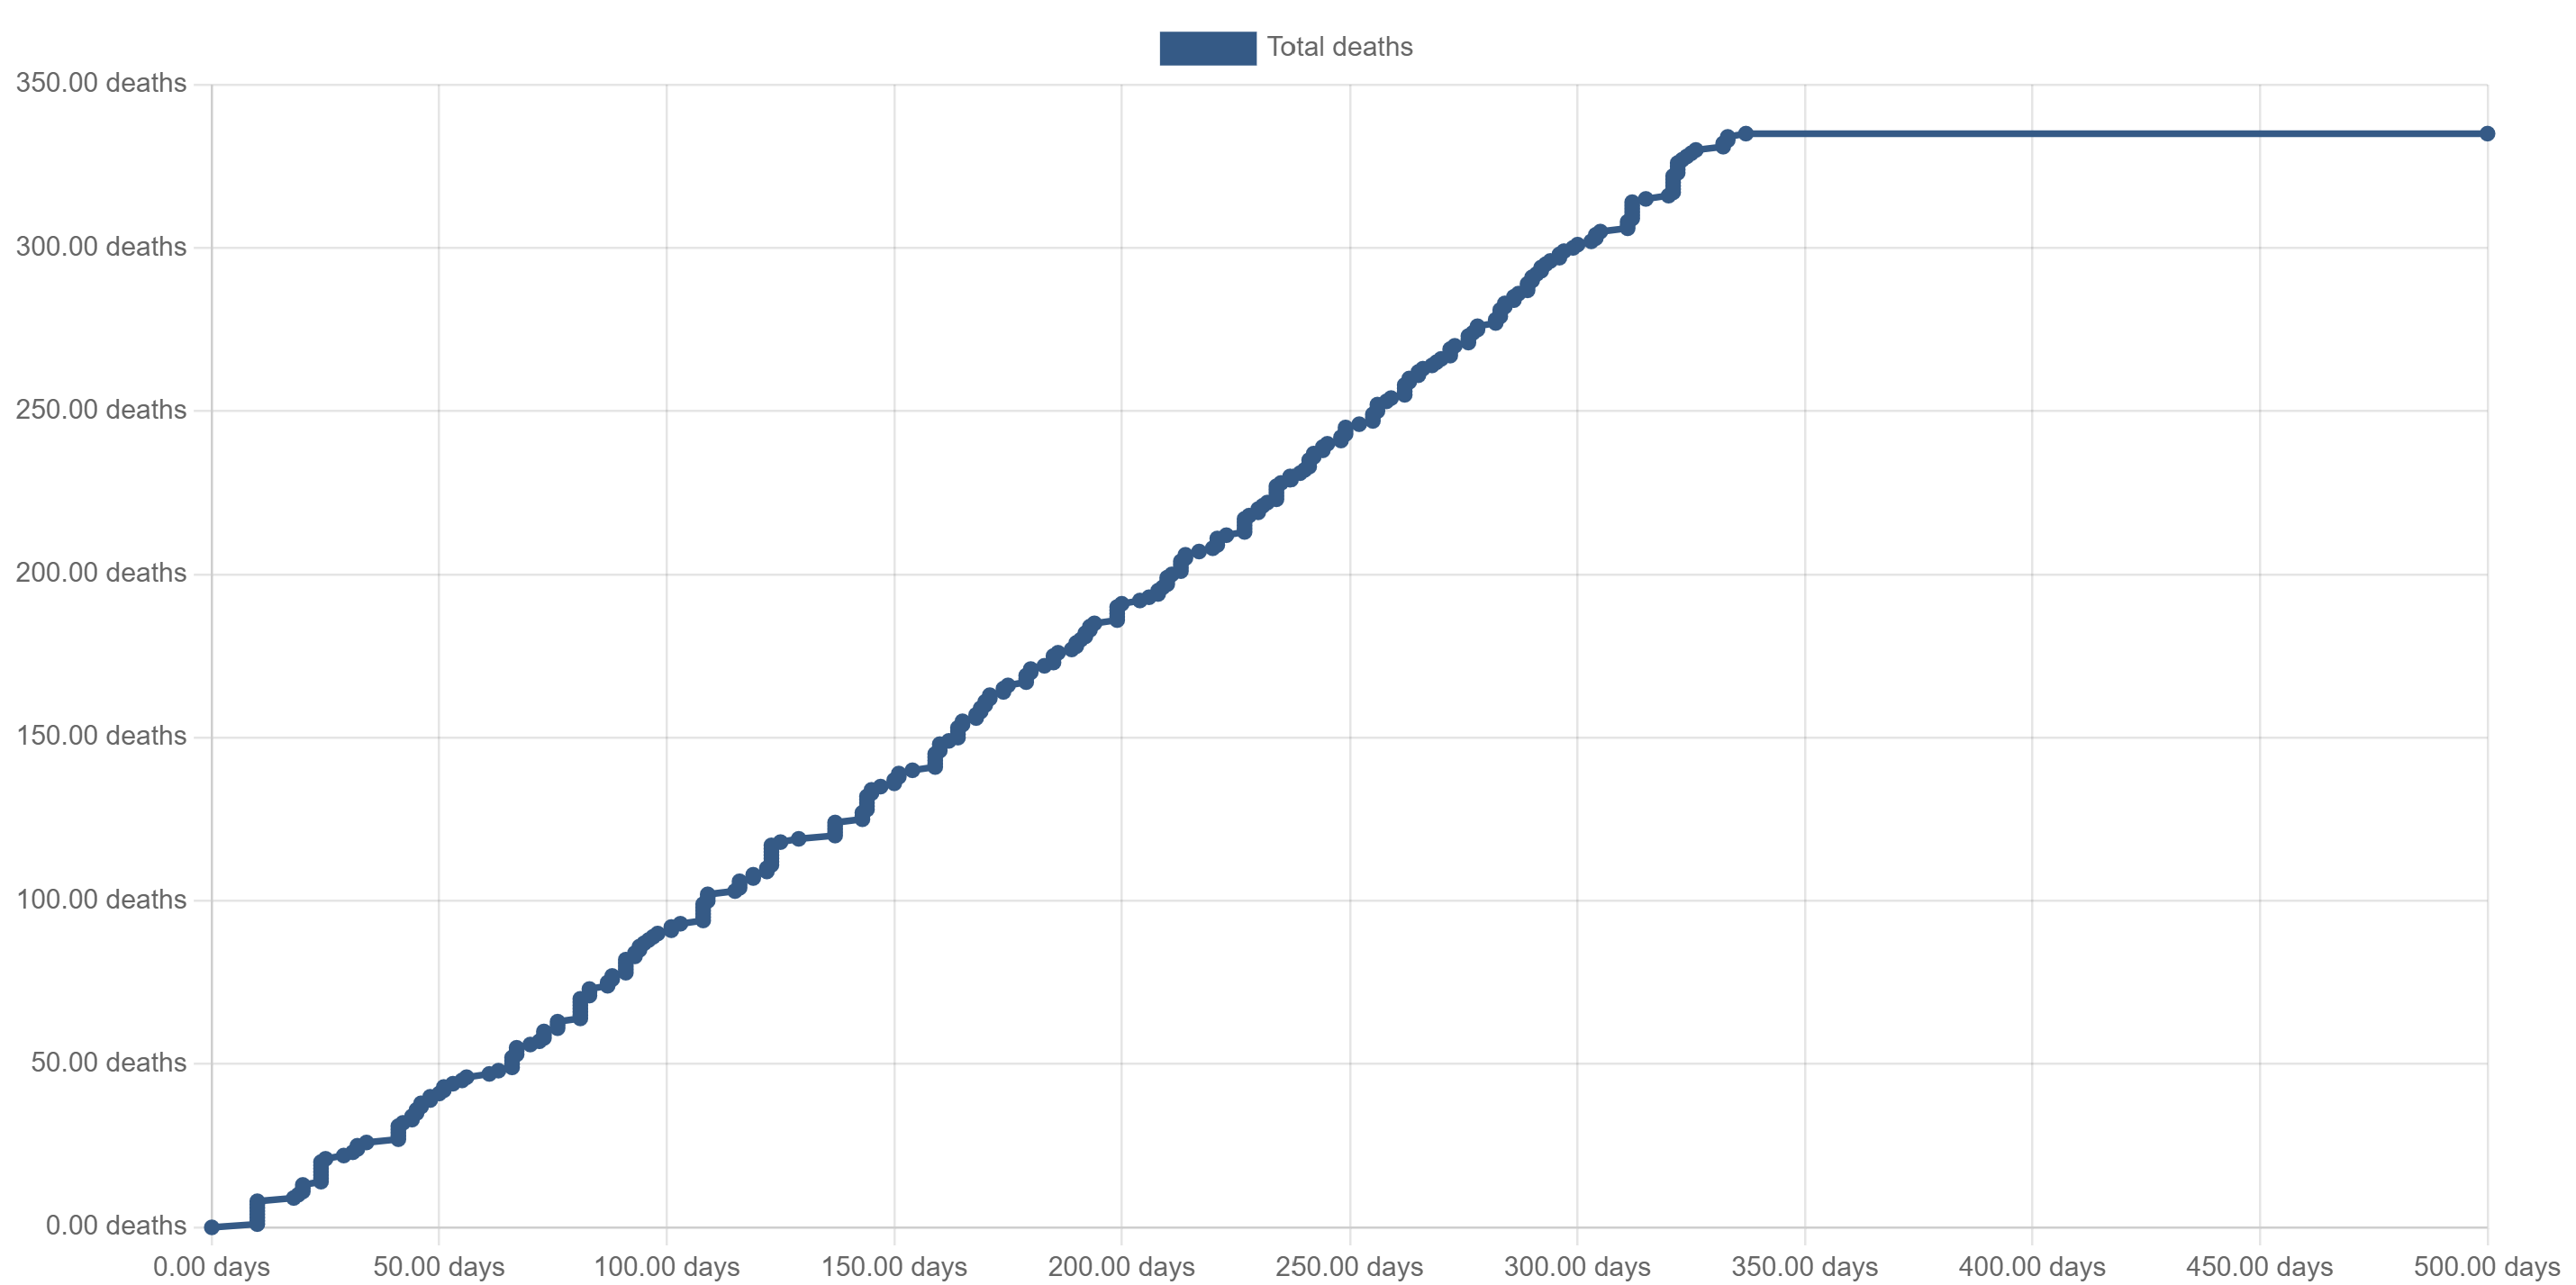
\includegraphics[width=0.8\textwidth]{007_team_5_agent_design/20-agent-2-food.png}
    \caption{Cumulative deaths per day for a 500 day simulation of 20 Team 5 agents with 2 food per agent}
    \label{fig:team5-20agents-2food}
\end{figure}

These results naturally led to the consideration of whether a homogeneous tower of Team 5 agents would achieve organisation given an infinite amount of time regardless of the number of agents provided at least two food per agent was available. We predict that this is not possible: every time an agent is replaced in the tower, its replacement is initialised with maximum selfishness and has no social network. It takes time for agents to build trust with each other but deaths occur too quickly for this happen if the settings of the tower are too strict.

\subsection*{Heterogeneous Tower Experiments}
These experiments compare the Team 5 agent with the agents designed by the other agent teams. The base parameters for all simulations are as follows:
\begin{itemize}
    \item 10 Team 5 agents, and two agents from each other team, excluding the random and selfish agents (i.e. half of the tower is Team 5).
    \item 6 food per agent
    \item 3 day reshuffle period
    \item 20 day simulation
\end{itemize}

\subsubsection*{Simulation Length}
\begin{figure}
    \centering
    \begin{minipage}{0.45\textwidth}
        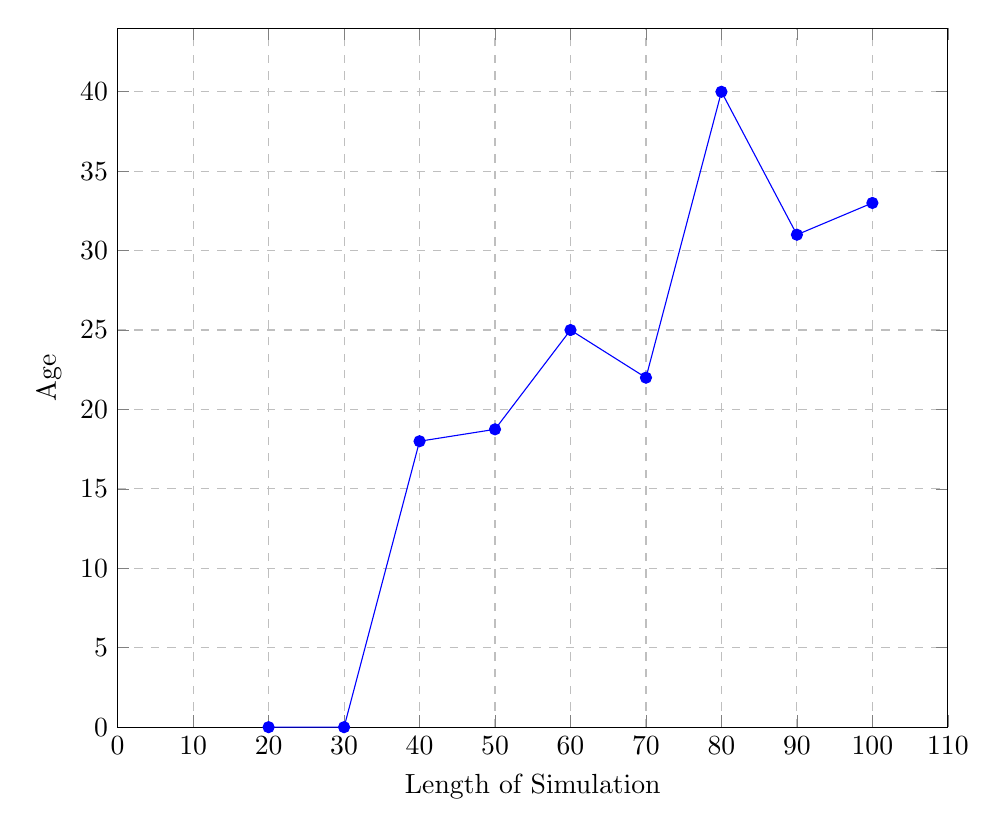
\begin{tikzpicture}
            \begin{axis}[
                width=\textwidth,
                ymin=0,
                xmin=0,
                xlabel=Length of Simulation,
                ylabel=Age,
                ymajorgrids=true,
                xmajorgrids=true,
                grid style=dashed,
            ]
            \addplot[mark=*,blue]
                coordinates{
                    (20, 0)
                    (30, 0)
                    (40, 18)
                    (50, 18.75)
                    (60, 25)
                    (70, 22)
                    (80, 40)
                    (90, 31)
                    (100, 33)
                };
            \end{axis}
            \end{tikzpicture}
            \caption{Average age upon death vs length of simulation. Points with age 0 mean no agent died during those simulations.}
            \label{fig:team5-exp-sim-length}
    \end{minipage}
    \hspace{0.05\textwidth}
    \begin{minipage}{0.45\textwidth}
        \begin{tikzpicture}
            \begin{axis}[
                width=\textwidth,
                ymin=0,
                xmin=0,
                xlabel=Food per agent,
                ylabel=Deaths,
                ymajorgrids=true,
                xmajorgrids=true,
                grid style=dashed,
            ]
            \addplot[mark=*,blue]
                coordinates{
                    (3, 7)
                    (4, 6)
                    (5, 2)
                    (6, 0)
                    (7, 1)
                };
            \end{axis}
            \end{tikzpicture}
            \caption{Number of deaths vs food per agent ratio}
            \label{fig:team5-exp-food-per-agent}
    \end{minipage}
\end{figure}
\ToDo{Check this result: is it actually true?}
Figure \ref{fig:team5-exp-sim-length} shows the relationship between the length of the simulation and the average age of Team 5 agents when they die: the graph shows a positive trend of increasing average age, implying that Team 5 agents perform better over time.

\subsubsection*{Food Per Agent}
Figure \ref{fig:team5-exp-food-per-agent} shows the effect of increasing the amount of food on the platform: the graph trends downwards as expected, showing that more food reduces the number of deaths.

\subsubsection*{Reshuffle Period}
Figure \ref{fig:team5-exp-reshuffle-period} shows the effect of changing the reshuffle period on the number of deaths. There is a small trend between deaths and the reshuffle period length, with an average increase in deaths of 0.25 per day; this implies that the agent performs better with a shorter reshuffle period.

\begin{figure}
    \centering
    \begin{minipage}{0.6\textwidth}
        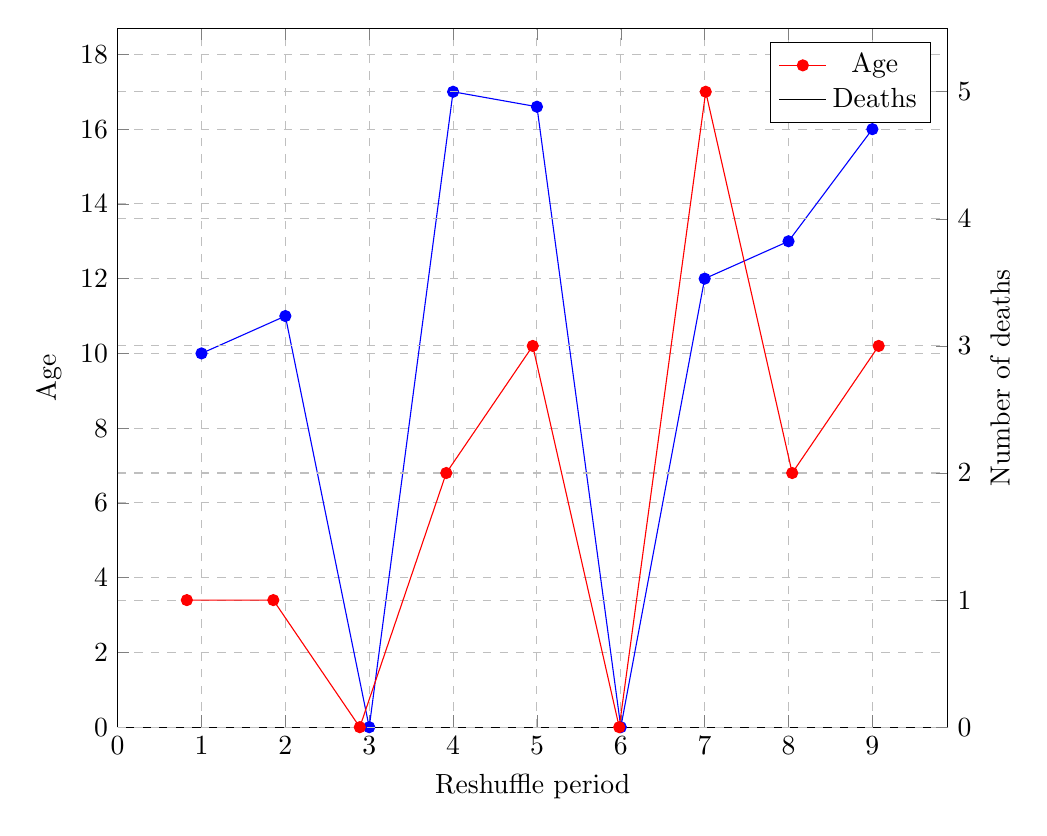
\begin{tikzpicture}
            \begin{axis}[
                width=\textwidth,
                axis y line*=left,
                ymin=0,
                xmin=0,
                xlabel=Reshuffle period,
                ylabel=Age,
                ymajorgrids=true,
                xmajorgrids=true,
                grid style=dashed,
            ]
            \addplot[mark=*,blue]
                coordinates{
                    (1, 10)
                    (2, 11)
                    (3, 0)
                    (4, 17)
                    (5, 16.6)
                    (6, 0)
                    (7, 12)
                    (8, 13)
                    (9, 16)
                }; \label{leg:team5-age}
            \addlegendentry{Age}
            \end{axis}
            
            \begin{axis}[
                width=\textwidth,
              axis y line*=right,
              axis x line=none,
              ymin=0,
              ylabel=Number of deaths,
              ymajorgrids=true,
              xmajorgrids=true,
              grid style=dashed,
            ]
            \addplot[mark=*,red]
                coordinates{
                    (1, 1)
                    (2, 1)
                    (3, 0)
                    (4, 2)
                    (5, 3)
                    (6, 0)
                    (7, 5)
                    (8, 2)
                    (9, 3)
                }; \label{leg:team5-deaths}
            \addlegendimage{/pgfplots/refstyle=leg:team5-age}\addlegendentry{Age}
            \addlegendimage{/pgfplots/refstyle=leg:team5-deaths}\addlegendentry{Deaths}
            \end{axis}
            \end{tikzpicture}
    \end{minipage}
    \caption{Average age upon death and number of deaths vs reshuffle period}
    \label{fig:team5-exp-reshuffle-period}
\end{figure}

% \subsection*{Comparing Team 5 with Other Agent Teams: Friend or Foe?}
% The next batch of experiments involved simulations with 10 Team 5 agents and 10 agents from another team to measure performance with other teams individually. Each of these experiments were run for 100 days, with the food per agent ratio varied to see how each agent type works together with varying food supply.

% We have highlighted those agents that work well with the Team 5 agent (``friends'') and those that do not (``foes''), given that one of the aims is to minimise the number of deaths in the tower. The chosen performance metrics are therefore the number of deaths and the average age upon death.

% \subsubsection*{Friends}
% Team 5 has the best survival rate when sharing the Tower with Team 4; simulations showed that with a food per agent ratio of 7 or 8, no deaths occurred within 100 days. Even when this ratio was 6 food per agent, there were only five deaths: three from Team 5 and two from Team 4, with average ages of 11.6 and 12.5 days upon death, respectively.

% Team 5 also performs well with Team 7 and Team 3; these results are shown in Tables \ref{tab:team5-team5-team7} and \ref{tab:team5-team5-team3}, respectively.

% \begin{table}
%     \centering
%     \begin{tabular}{|c|c|c|c|}
%         \hline
%         \textbf{Food per agent ratio} & \textbf{6} & \textbf{7} & \textbf{8}\\
%         \hline
%         Team 5 deaths and average age upon death       & 4, 46 & 0, 0 & 0, 0\\
%         \hline
%         Team 7 deaths and average age upon death       & 4, 19.5 & 3, 25 & 1, 22\\
%         \hline
%     \end{tabular}
%     \caption{Results of a Tower consisting of Team 5 and Team 7 agents}
%     \label{tab:team5-team5-team7}
% \end{table}

% \begin{table}
%     \centering
%     \begin{tabular}{|c|c|c|c|}
%         \hline
%         \textbf{Food per agent ratio} & \textbf{6} & \textbf{7} & \textbf{8}\\
%         \hline
%         Team 5 deaths and average age upon death       & 11, 41 & 7, 63 & 1, 15\\
%         \hline
%         Team 3 deaths and average age upon death       & 8, 45 & 0, 0 & 0, 0 \\
%         \hline
%     \end{tabular}
%     \caption{Results of a Tower consisting of Team 5 and Team 3 agents}
%     \label{tab:team5-team5-team3}
% \end{table}

% \subsubsection*{Foes}
% Team 5 does not perform well with either Team 6 or Team 2. When paired with Team 6, the Team 6 agents die often and have less than half the lifespan of the Team 5 agents. This issue persists with increased amount of food on the platform.

% When paired with Team 2, the Team 2 agent has significantly fewer deaths than the Team 5 agent and also has a longer lifespan. These results suggest that this agent pairing is unable to self-organise, with the potentially more selfless Team 5 agents left to starve by the Team 2 agents. This is because the Team 2 agents do not communicate except to ask for the HP of other agents.

% The Team 5 agent is least compatible with random agents (i.e. agents which take a random amount of food). The total number of deaths is highest and average age upon death is lowest with this pairing. The life expectancy also does not improve with more food on the platform.

\subsection*{Self-Organisation With Other Agents}
The overall aim within the tower is for agents to self-organise and create a stable society. Tests were run to investigate how compatible the Team 5 agent is with each of the agents designed by each of the other teams. Simulations were run with a tower consisting of Team 5 agents and one other agent type, with seven agents each and five food available per agent, to see whether they could self-organise within 100 days. These results are shown in Table \ref{tab:team5-self-org-agents}.

Team 5 is able to self-organise with Teams 3, 4, and 7, and can do so immediately with Team 4. Team 5 does not perform well with either Teams 2 or 6; the agents were not able to self-organise within 100 days, resulting in continual deaths.

The Team 5 agent also does not perform well with random agents (i.e. agents which take a random amount of food). Experiments on towers consisting of Team 5 and random agents resulted in a comparatively high number of deaths, with a low average age upon death. The average age also does not improve when the food per agent ratio is increased.

\begin{table}
    \centering
    \begin{tabular}{|c|c|c|c|c|c|}
        \hline
        \textbf{Agent type} & \textbf{Team 2} & \textbf{Team 3}& \textbf{Team 4} & \textbf{Team 6} & \textbf{Team 7}\\
        \hline
        Team 5 deaths & 25 & 5 & 0 & 25 & 12 \\
        \hline
        Other agent deaths & 19 & 5 & 0 & 35 & 8 \\
        \hline
        Organisation? & NO & 67 days & 0 days & NO & 62 days \\
        \hline
    \end{tabular}
    \caption{Team 5 interactions with other agents}
    \label{tab:team5-self-org-agents}
\end{table}

\section{Conclusion}\label{sec:team5-conclusion}
The Team 5 agent is capable of achieving self-organisation within the tower provided the simulation parameters are not too strict. A large number of agents within the tower greatly inhibits the agent's ability to self-organise, but for low agent numbers, they are capable of organising when the food per agent ratio is at least 2. This demonstrates the reliance on communication and sharing of knowledge in order to solve the problem of long-term survival in the tower.

During the presentation for this coursework, Professor Pitt compared the Team 5 agent's strategy to theory from Ober, who stated that ``alignment is an epistemic process, predicated on the right people having and using the right information in the right context'' \cite{ober_athens}. We had not considered this theory when designing our agent, however in a sort of convergent evolution we observed this in the randomeness and large variation in the Team 5 agent's ability to self-organise, and the conditions required for this to be successful.
